\documentclass{beamer}

\usepackage[utf8]{inputenc}

\usepackage{default}
\usepackage{hyperref}
\usepackage{graphicx}
\usepackage{listings}
\usepackage{tikz}

\newcommand*{\email}[1]{
	\href{mailto:#1}{#1}
}

\title{Approaches to apply Symbolic Execution in non-sequential applications}
\author{Savu Victor-Gabriel}
\institute{Technische Universität München, \email{victorsavu3@gmail.com}}

\definecolor{Paper1Color}{RGB}{221, 224, 204}
\definecolor{Paper2Color}{RGB}{191, 227, 224}
\definecolor{Paper3Color}{RGB}{196, 198, 231}
\definecolor{Paper4Color}{RGB}{239, 201, 185}
\definecolor{White}{RGB}{255, 255, 255}

\definecolor{Paper1Full}{RGB}{181, 137, 0}
\definecolor{Paper2Full}{RGB}{42, 161, 152}
\definecolor{Paper3Full}{RGB}{108, 113, 196}
\definecolor{Paper4Full}{RGB}{203, 75, 22}


\begin{document}
	\frame{\titlepage}
	
	\begin{frame}
		\frametitle{Table of Contents}
		\tableofcontents
	\end{frame}
	
	\section{Concepts}
	
	\begin{frame}
		\frametitle{Symbolic execution}
		
		\begin{figure}[htbp]
			\centering
			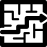
\includegraphics[scale=0.1]{exit}
		\end{figure}
		
		\begin{itemize}
			\item Symbolic values
			\item Path condition
			\item Limitations
			\begin{itemize}
				\item Path explosion
				\item Unbounded input
				\item Floating point values
			\end{itemize}
		\end{itemize}
	\end{frame}
	
	\begin{frame}
		\frametitle{Scheduling}
		
		\begin{figure}[htbp]
			\centering
			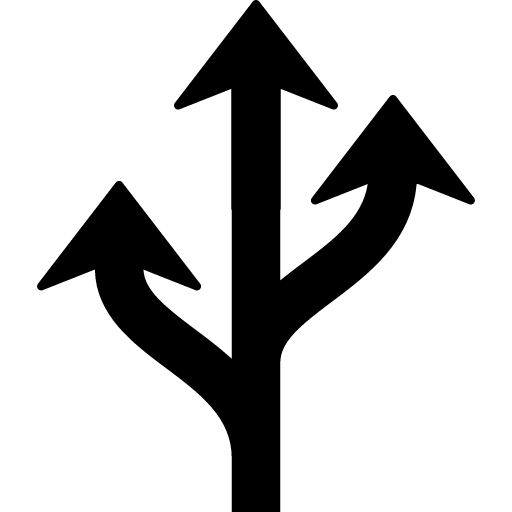
\includegraphics[scale=0.1]{schedule}
		\end{figure}
		
		\begin{itemize}
			\item Thread interleaving
			\item Scheduler choices
			\begin{itemize}
				\item Thread wake-up
				\item Preemptions
			\end{itemize}
			\item Problems
			\begin{itemize}
				\item Path explosion when dealing with threads
			\end{itemize}
		\end{itemize}
	\end{frame}
	
	\begin{frame}
		\frametitle{Concolic testing}
		
		\begin{figure}[htbp]
			\centering
			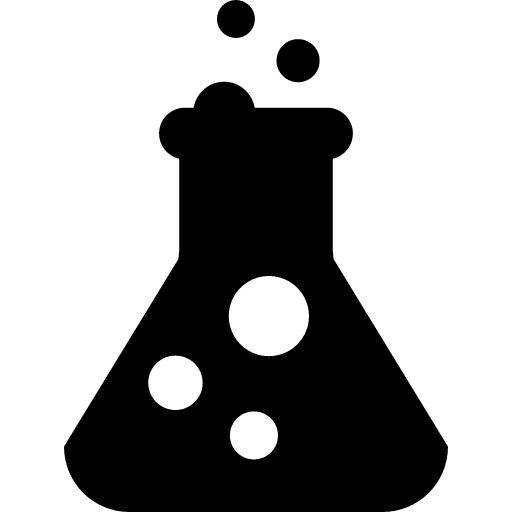
\includegraphics[scale=0.1]{concolic}
		\end{figure}
		
		\begin{itemize}
			\item Very practical approach
			\item Uses actual input to run a program
			\item Attempts to generate new input for further runs
			\item Problems
			\begin{itemize}
				\item Is not always complete (not all constraints can be solved)
				\item Finding inputs can be harder than standard symbolic execution
			\end{itemize}
		\end{itemize}
	\end{frame}
	
	\section{Approaches}
	
	%\subsection{Parallel Symbolic Execution for Automated Real-World Software Testing \cite{base3}}
	
	\setbeamercolor{background canvas}{bg=Paper1Color}
	
	\begin{frame}
		\frametitle{1. Parallel Symbolic Execution for Automated Real-World Software Testing \cite{base3}}
		
		\begin{figure}[htbp]
			\centering
			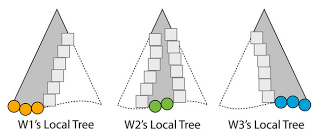
\includegraphics[scale=0.5]{cloud9}
		\end{figure}
		
		\begin{itemize}
			\item Method designed to test actual software
			\item Based on KLEE
			\item Extended POSIX support
			\item Distributed execution engine
			\item Simple to use
		\end{itemize}
	\end{frame}
	
	\begin{frame}
		\frametitle{Parallel Symbolic Execution for Automated Real-World Software Testing \cite{base3}}
		
		\begin{itemize}
			\item Not focused on concurrent software
			\item Depth of analysis can be selected for each test
			\begin{itemize}
				\item Complete analysis
				\item Iterative context bounding
				\item No preemption
				\item Deterministic scheduling (default)
			\end{itemize}
			\item Full POSIX threads support
		\end{itemize}
	\end{frame}
	
	\begin{frame}
		\frametitle{Iterative context bounding \cite{Musuvathi}}
		
		\begin{figure}[htbp]
			\centering
			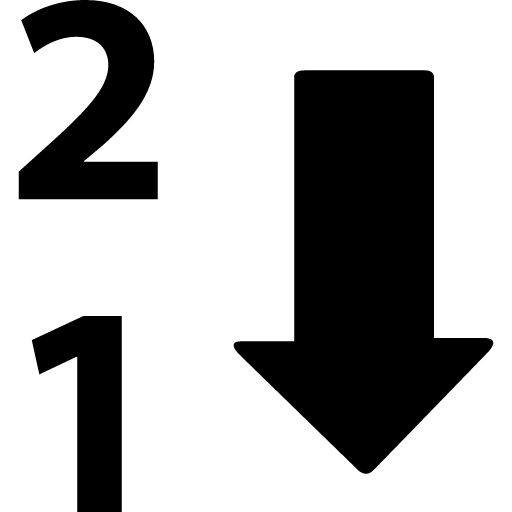
\includegraphics[scale=0.1]{limit}
		\end{figure}
		
		\begin{itemize}
			\item Simple search strategy
			\item Limits the number of preemtions
			\item Normal execution is not affected
			\item Very likely to find most bugs
		\end{itemize}
	\end{frame}
	
	%\subsection{Concolic Testing of Multithreaded Programs and	Its Application to Testing Security Protocols \cite{base4}}
	\setbeamercolor{background canvas}{bg=Paper2Color}
	
	\begin{frame}
		\frametitle{2. Concolic Testing of Multithreaded Programs and	Its Application to Testing Security Protocols \cite{base4}}
		
		\begin{itemize}
			\item Focused on reducing execution time of the analysis
			\item Implementation based on DVC
			\item Uses concolic testing for both input and scheduling
		\end{itemize}
	\end{frame}
	
	\begin{frame}
		\frametitle{Dynamic vector clocks (DVC) \cite{dvcproof}}
		
		\begin{figure}[htbp]
			\centering
			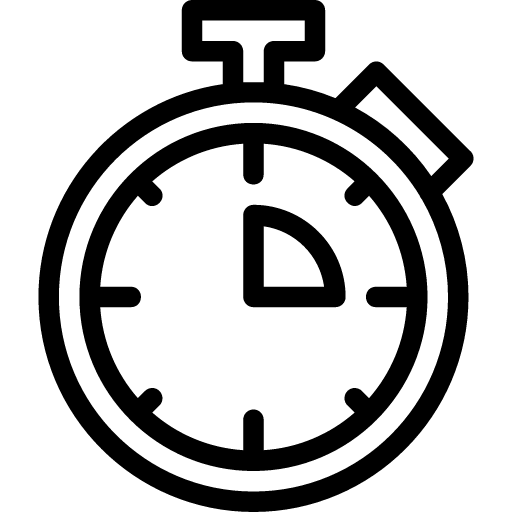
\includegraphics[scale=0.1]{clock}
		\end{figure}
		
		\begin{itemize}
			\item Detect possible race conditions
			\item Make analysis complete without the need to process all thread interleavings
			\item Easily computed during concolic execution
			\item Races can be fliped by postponing
		\end{itemize}
	\end{frame}

\defverbatim[colored]\lstI{
		\begin{lstlisting}[mathescape,tabsize=2,basicstyle=\tiny]
compute_next_input_and_schedule(n, input, path, branch_hist)
	for j in n-1..0
		if path[j] has a event
			if number of posponed threads < enabled threads
				if path[j] has a race with a future event
					add current thread to posponed threads in path[j]
					change thread of path[j] to a different one
					shorten path, branch_hist to j elements
					return (input, path, branch_hist, false)
		else
			flip branch_hist[j]
			if $\exists$ input2 that satisfies branch_hist
				shorten path, branch_hist to j elements
				return (input2, path, branch_hist, false)
	return ([],[],[], true);
		
		\end{lstlisting}
}
	
	
	\begin{frame}[fragile]
		\frametitle{Algorithm}

		\lstI
	\end{frame}
	
	%\subsection{Generalized Symbolic Execution for Model Checking and Testing \cite{base5}}
	\setbeamercolor{background canvas}{bg=Paper3Color}
	
	\begin{frame}
		\frametitle{3. Generalized Symbolic Execution for Model Checking and Testing \cite{base5}}
		
		\begin{itemize}
			\item Can deal with \textbf{unbounded} input
			\item Uses Java PathFinder as a model checker
			\item Exhaustive search of all interleavings
		\end{itemize}
	\end{frame}
	
	\begin{frame}
		\frametitle{Generalized Symbolic Execution for Model Checking and Testing \cite{base5}}
		
		\begin{figure}[htbp]
			\centering
			\includegraphics[bb=1.8in 6.5in 7.5in 9.5in,clip,page=3,scale=0.9]{GSE.pdf}
		\end{figure}
	\end{frame}
	
	%\subsection{GKLEE: concolic verification and test generation for GPUs \cite{base7}}
	\setbeamercolor{background canvas}{bg=Paper4Color}
	
	\begin{frame}
		\frametitle{4. GKLEE: concolic verification and test generation for GPUs \cite{base7}}
		
		\begin{itemize}
			\item Specialized implementation for CUDA devices
			\item Scales very well to a very large number of threads
			\item Detects most concurrency errors and performance bottlenecks
		\end{itemize}
	\end{frame}
	
	\begin{frame}
		\begin{figure}[htbp]
			\centering
			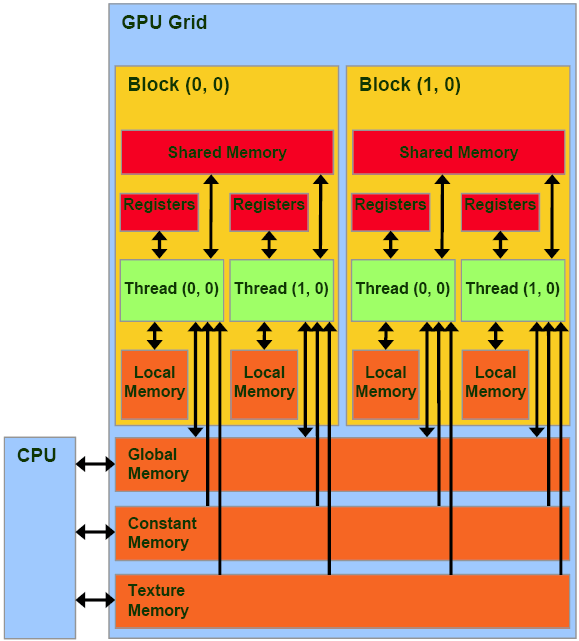
\includegraphics[scale=0.4]{CUDA-memory-model}
		\end{figure}
	\end{frame}
	
	\begin{frame}
		\frametitle{Approach}
		\begin{itemize}
			\item Takes advantage of hardware characteristics
			\begin{itemize}
				\item No preemptions
				\item SIMT
				\item Barriers are the only synchronization primitives
			\end{itemize}
			\item Results
			\begin{itemize}
				\item Deadlock
				\item Intra/Inter Race conditions
				\item Global races
				\item Access patterns
				\item Missing volatile
			\end{itemize}
		\end{itemize}
	\end{frame}
	
	\setbeamercolor{background canvas}{bg=White}
	
	\section{Comparison}
	
	\begin{frame}
		\frametitle{Comparison}
		
		\begin{figure}[htbp]
			\centering
			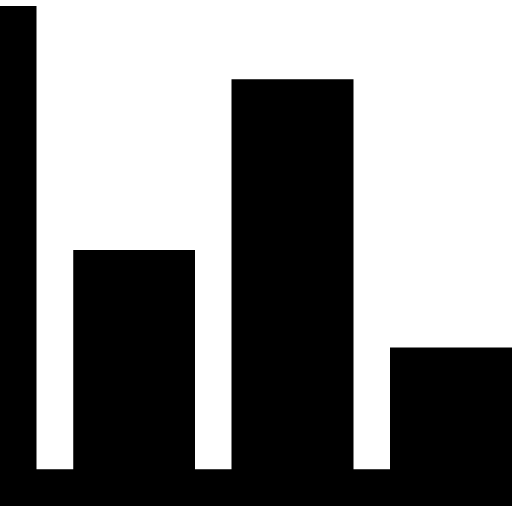
\includegraphics[scale=0.1]{comparison}
		\end{figure}
		
		\begin{itemize}
			\item Method
			\begin{itemize}
				\color{Paper1Full} \setbeamercolor{item}{fg=Paper1Full} \item[1.] Concolic testing
				\color{Paper2Full} \setbeamercolor{item}{fg=Paper2Full} \item[2.] Concolic testing
				\color{Paper3Full} \setbeamercolor{item}{fg=Paper3Full} \item[3.] Model checking
				\color{Paper4Full} \setbeamercolor{item}{fg=Paper4Full} \item[4.] Concolic testing
			\end{itemize}
		\end{itemize}
	\end{frame}
	
	\begin{frame}
		\frametitle{Comparison II}
		
		\begin{itemize}
			\item Goal
			\begin{itemize}
				\color{Paper4Full} \setbeamercolor{item}{fg=Paper4Full} \item[4.] Testing/Performance
			\end{itemize}
			\item Required skill
			\begin{itemize}
				\color{Paper1Full} \setbeamercolor{item}{fg=Paper1Full} \item[1.] Very low
			\end{itemize}
			\item Automation
			\begin{itemize}
				\color{Paper1Full} \setbeamercolor{item}{fg=Paper1Full} \item[1.] Full
				\color{Paper2Full} \setbeamercolor{item}{fg=Paper2Full} \item[2.] Full
				\color{Paper3Full} \setbeamercolor{item}{fg=Paper3Full} \item[3.] Full
				\color{Paper4Full} \setbeamercolor{item}{fg=Paper4Full} \item[4.] Full
			\end{itemize}
			\item Applicability
			\begin{itemize}
				\color{Paper1Full} \setbeamercolor{item}{fg=Paper1Full} \item[1.] POSIX
				\color{Paper2Full} \setbeamercolor{item}{fg=Paper2Full} \item[2.] Java
				\color{Paper3Full} \setbeamercolor{item}{fg=Paper3Full} \item[3.] Java
				\color{Paper4Full} \setbeamercolor{item}{fg=Paper4Full} \item[4.] CUDA
			\end{itemize}
		\end{itemize}
	\end{frame}
	
	\begin{frame}
		\frametitle{Concurrency}
		
		\begin{itemize}
			\item Scalability to multiple threads
			\begin{itemize}
				\color{Paper1Full} \setbeamercolor{item}{fg=Paper1Full} \item[1.] allows more computing power
				\color{Paper4Full} \setbeamercolor{item}{fg=Paper4Full} \item[4.] very good
			\end{itemize}
			\item Scalability to bigger input
			\begin{itemize}
				\color{Paper1Full} \setbeamercolor{item}{fg=Paper1Full} \item[1.] allows more computing power
				\color{Paper3Full} \setbeamercolor{item}{fg=Paper3Full} \item[3.] very bad
				\color{Paper4Full} \setbeamercolor{item}{fg=Paper4Full} \item[4.] good
			\end{itemize}
		\end{itemize}
	\end{frame}
	
	\begin{frame}
		\frametitle{Concurrency II}
		
		\begin{itemize}
			\item Complete analysis
			\begin{itemize}
				\color{Paper1Full} \setbeamercolor{item}{fg=Paper1Full} \item[1.] Optinal
				\color{Paper2Full} \setbeamercolor{item}{fg=Paper2Full} \item[2.] Unlikely
				\color{Paper3Full} \setbeamercolor{item}{fg=Paper3Full} \item[3.] Yes/Slow
				\color{Paper4Full} \setbeamercolor{item}{fg=Paper4Full} \item[4.] Yes
			\end{itemize}
			\item Partial results
			\begin{itemize}
				\color{Paper1Full} \setbeamercolor{item}{fg=Paper1Full} \item[1.] Yes
				\color{Paper2Full} \setbeamercolor{item}{fg=Paper2Full} \item[2.] Yes
				\color{Paper3Full} \setbeamercolor{item}{fg=Paper3Full} \item[3.] No
				\color{Paper4Full} \setbeamercolor{item}{fg=Paper4Full} \item[4.] No
			\end{itemize}
		\end{itemize}
	\end{frame}
	
	\section{Conclusions}
	
	\begin{frame}
		\frametitle{Conclusions}
		
		\begin{itemize}
			\item Many developments
			\item No one best approach, but most methods can be combined
			\item Hopefully more research in the field
		\end{itemize}
	\end{frame}
	
	\begin{frame}
		Questions
	\end{frame}
	
	\section{References}
	
	\begin{frame}
		\frametitle{References}
		\tiny
		\bibliographystyle{splncs03}
		\bibliography{ref}
	\end{frame}
\end{document}
